%%---------------------------------------------------------------------------%%
%% draco-6_2_0.tex
%% Thomas M. Evans
%% $Id$
%%---------------------------------------------------------------------------%%
\documentclass[note]{ResearchNote_pdf}
\usepackage[centertags]{amsmath}
\usepackage{amssymb,amsthm,graphicx}
\usepackage[mathcal]{euscript}
\usepackage{tabularx}
\usepackage{cite}
\usepackage{c++}
\usepackage{tmadd,tmath}
\usepackage{listings}
\usepackage{color}
% \usepackage{url}
\usepackage{hyperref}

%%---------------------------------------------------------------------------%%
%% DEFINE SPECIFIC ENVIRONMENTS HERE
%%---------------------------------------------------------------------------%%
%\newcommand{\elfit}{\ensuremath{\operatorname{Im}(-1/\epsilon(\vq,\omega)}}
%\msection{}-->section commands
%\tradem{}  -->add TM subscript to entry
%\ucatm{}   -->add trademark footnote about entry

\newcommand{\draco}{Draco}
\newcommand{\dracor}{\draco-6\_2\_0}
\newcolumntype{L}{>{\ttfamily}X}

%\newcommand{\autoconf}{\textsf{Autoconf}}
%\newcommand{\automake}{\textsf{Automake}} 
\newcommand{\cmake}{\textsf{CMake}}
\newcommand{\ctest}{\textsf{CTest}}
\newcommand{\cdash}{\textsf{CDash}}
\newcommand{\scons}{\textsf{SCons}}
\newcommand{\CVS}{\textsf{CVS}}  
\newcommand{\make}{\textsf{Make}}
\newcommand{\gpp}{\textsf{g++}}

\newcommand{\tableText}[1]{{\raggedright #1}}


\definecolor{listingBG}{rgb}{0.95,0.95,0.95}

%% \lstset{language=sh,
%%   showstringspaces=false,
%%   frame=shadowbox,
%%   basicstyle=\footnotesize,
%%   rulesepcolor=\color{black},
%%   backgroundcolor=\color{listingBG}
%% }

\hypersetup{
    bookmarks=true,         % show bookmarks bar?
    unicode=false,          % non-Latin characters in Acrobat’s bookmarks
    pdftoolbar=true,        % show Acrobat’s toolbar?
    pdfmenubar=true,        % show Acrobat’s menu?
    pdffitwindow=false,     % window fit to page when opened
    %pdfstartview={FitH},    % fits the width of the page to the window
    %pdftitle={My title},    % title
    %pdfauthor={Author},     % author
    %pdfsubject={Subject},   % subject of the document
    %pdfcreator={Creator},   % creator of the document
    %pdfproducer={Producer}, % producer of the document
    %pdfkeywords={keyword1} {key2} {key3}, % list of keywords
    pdfnewwindow=true,      % links in new window
    colorlinks=false,       % false: boxed links; true: colored links
    linkcolor=red,          % color of internal links
    citecolor=green,        % color of links to bibliography
    filecolor=magenta,      % color of file links
    urlcolor=cyan           % color of external links
}

%%---------------------------------------------------------------------------%%
%% BEGIN DOCUMENT
%%---------------------------------------------------------------------------%%
\begin{document}

%%---------------------------------------------------------------------------%%
%% OPTIONS FOR NOTE
%%---------------------------------------------------------------------------%%

\toms{Distribution}
%\toms{Joe Sixpak/XTM, MS B226}
\refno{CCS--2:11--XX (U)}
\subject{Release of \dracor}

%-------NO CHANGES
\divisionname{Computer, Computational and Statistical Sciences}
\groupname{CCS--2:Computational Physics \& Methods}
\fromms{Kelly Thompson/CCS--2 D409} % \\
%  Jae Chang/CCS--2 D409}
\phone{(505)665--8090}
\originator{kgt}
\typist{kgt}
\date{07/31/2011}
%-------NO CHANGES

%-------OPTIONS
%\reference{NPB Star Reimbursable Project}
%\thru{P. D. Soran, XTM, MS B226}
%\enc{list}      
%\attachments{list}
%\cy{list}
%\encas
%\attachmentas
%\attachmentsas 
%-------OPTIONS

\revisionnum{1}

%%---------------------------------------------------------------------------%%
%% DISTRIBUTION LIST
%%---------------------------------------------------------------------------%%

\distribution {

  Baker, Randal,      CCS--2  MS D409\\ 
  Budge, Kent,        CCS--2  MS D409\\
%  Buksas, Michael     CCS--7  MS B287\\
  Chang, Jae,         CCS--2  MS D409\\
  Dahl, Jon,          CCS--2  MS D409\\ 
  Densmore, Jeffery,  CCS--2  MS D409\\ 
  Fichtl, Erin,       CCS--2  MS D409\\
%  Hungerford, Aimee,  XTD--6  MS T085\\  
  Lowrie, Robert,     CCS--2  MS D413\\ 
  Rockerfeller, Gabe  CCS--2  MS D409\\
  Rosa, Massimiliano, CCS--2  MS D409\\
  Thompson, Kelly,    CCS--2  MS D409\\ 
  Turner, Scott,      CCS--2  MS D409\\ 
  Urbatsch, Todd,     CCS--2  MS D409\\ 
  Warsa, James,       CCS--2  MS D409\\ 
  Wollaber, Allan,    CCS--2  MS D409\\
  Zerr, Robert,       CCS--2  MS D409\\
}

%%---------------------------------------------------------------------------%%
%% BEGIN NOTE
%%---------------------------------------------------------------------------%%

\opening

\begin{abstract}
  
  We have released \dracor.  This release marks significant changes to
  \draco.  First and foremost, one new component has been added to
  \draco.  The \textsf{device} component provides a generic driver
  interface that will be used for controlling the DACS on RoadRunner.
  One component, \textsf{xm} has been retired from \draco. The
  \textsf{plot2D}, \textsf{cdi\_eospac} and \textsf{pcgWrap}
  components are not under active development and are not provided
  with this release. The code base was updated to elminate warnings
  issued by \gpp.  Additional changes have been made to the
  \draco\ environment, organization, build system, and automatic
  documentation system, including the adoption of the \cmake-toolset
  (\cmake, \ctest, and \cdash) as the only fully supported build
  system for \draco.
\end{abstract}

%%---------------------------------------------------------------------------%%

\section{\draco\ Contributors}

The following people are contributors to \draco:
\begin{center}
  \small
  \begin{tabular}{ll}
    Allan Wollaber    & \texttt{wollaber@lanl.gov} \\
    Gabe Rockerfeller & \texttt{gaber@lanl.gov} \\
    Jae Chang         & \texttt{jhchang@lanl.gov} \\
    Jeff Densmore     & \texttt{jdd@lanl.gov} \\
    Jim Warsa         & \texttt{warsa@lanl.gov} \\
    Kelly Thompson    & \texttt{kgt@lanl.gov} \\
    Kent Budge        & \texttt{kgbudge@lanl.gov} \\
    Mike Buksas       & \texttt{mwbuksas@lanl.gov} \\
    Rob Lowrie        & \texttt{lowrie@lanl.gov} \\
    Ryan McClarren    & \texttt{rgm@tamu.edu} \\
    Seth R. Johnson   & \texttt{sethajoh@umich.edu} \\
    Tim Kelley        & \texttt{tkellyt@lanl.gov} \\
    Todd Urbatsch     & \texttt{tmonster@lanl.gov} \\
    Tom Evans         & \texttt{evanstm@ornl.gov} \\
  \end{tabular}
\end{center}

%%---------------------------------------------------------------------------%%
\newpage
\section{\draco\ Component Packages}

\dracor\ contains the following component packages:
\begin{center}
  \footnotesize
  \begin{tabular}{lp{4.0in}}
    \hline\hline
    \textsf{RTT\_Format\_Reader} & \tableText{\textsf{meshReaders}
      implementation for RTT format meshes} \\
    \textsf{c4} & \tableText{communication library for message passing interface (MPI)} \\
    \textsf{cdi} & \tableText{Common Data Interface (CDI) component} \\
    \textsf{cdi\_analytic} & \tableText{CDI analytic data component} \\
    \textsf{cdi\_gandolf} & \tableText{CDI GANDOLF wrapper for loading
      opacities from IPCRESS files~\cite{gandolf,tops}} \\
    \textsf{device}         & \tableText{Minimal representation of the
      host side of a hybrid process (i.e.: DACS)} \\
    \textsf{diagnostics}  & \tableText{CPP macros for controlling runtime
      verbosity and inline timing of function calls} \\
    \textsf{ds++}         & \tableText{data structures library, DbC,
      low level functions, etc.} \\
    \textsf{fit}          & \tableText{least squares fitting routines} \\
    \textsf{fpe\_trap}    & \tableText{catch floating point signals and throw
      C++ exceptions} \\
    \textsf{lapack\_wrap} & \tableText{C++ wrapper to BLAS and LAPACK} \\
    \textsf{linear}       & \tableText{direct solvers for small linear systems} \\
    \textsf{meshReaders}  & \tableText{mesh reader interface} \\
    \textsf{mesh\_element} & \tableText{defines fundamental mesh element types
      used by \textsf{meshReaders} and \textsf{RTT\_Format\_Reader}} \\
    \textsf{min}          & \tableText{locate function minimums} \\
    \textsf{norms}        & \tableText{compute norms of vectors} \\
    \textsf{ode}          & \tableText{Runge\_Kutta, etc.} \\
    \textsf{parser}       & \tableText{generic input parser} \\
    \textsf{quadrature}   & \tableText{quadrature component} \\
    \textsf{rng}          & \tableText{random number generators} \\
    \textsf{roots}        & \tableText{root finding algorithms} \\
    \textsf{shared\_lib}  & \tableText{dynamic loading of shared libraries} \\
    \textsf{special\_functions} & \tableText{math functions not provided by the
      C++ standardard library} \\
    \textsf{timestep}     & \tableText{a timestep controller component} \\
    \textsf{traits}       & \tableText{traits used by other \draco\ components} \\
    \textsf{units}        & \tableText{a physics units component} \\
    \textsf{viz}          & \tableText{interfaces to visualization tools (EnSight)} \\
    \hline\hline 
  \end{tabular}
\end{center}

%%---------------------------------------------------------------------------%%

\section{\draco\ Toolset changes}
\subsection{\draco\ build tools}

As of this release \draco's only supported configure system is
\cmake\cite{cmake}.  Deprecated autoconf and \scons\ files will be
retired over the next few months.  The current release relies on
features (e.g.: \texttt{FindMPI.cmake}) only found in \cmake-2.8.5 or
newer.

\cmake\ was selected because it has mature cross platform support and
can construct build projects for various systems (\textsf{Makefiles},
\textsf{XCode}, \textsf{Eclipse}, \textsf{Visual Studio}, etc.).
\cmake\ also has an excellent dependency generator for both source
code and tests allowing multi-threaded builds (e.g.: \texttt{make
  -j16}) to make the most of available hardware.  \cmake\ has provides
online\footnote{http://www.cmake.org/cmake/help/documentation.html}
and command line documentation (\texttt{cmake --help}). A tutorial is
also available at
\url{http://www.cmake.org/cmake/help/cmake_tutorial.html}.


Using \cmake\ can be similar to using the old autoconf build system.
For example, draco can be compiled using commands similar to these:

\lstset{language=ksh, %C++,
  showstringspaces=false,
  frame=shadowbox,
  basicstyle=\footnotesize,
  rulesepcolor=\color{black},
  backgroundcolor=\color{listingBG}
}
\begin{lstlisting}[basicstyle=\footnotesize,
    xleftmargin=1.0in, xrightmargin=1.0in]
% install -d $build_dir
% cd $build_dir
% cmake [-D<OPTION>=<VALUE> ... ] $source_dir
% make -j4
% ctest -j4
% make -j4 install
\end{lstlisting}

For developers more comfortable with GUI environments, \cmake\ can be
started as a stand alone GUI (e.g.: \texttt{cmake-gui} or
\texttt{ccmake}). 

\subsubsection{List of configure options}

There are many options that control the build configuration.  A few of
the more important ones are listed below.

\begin{center}
  \footnotesize
  \begin{tabular}{lp{4.0in}}
    \hline\hline
    % ----------------------------------------
    \texttt{CMAKE\_INSTALL\_PREFIX} & \tableText{Directory location for installing
      libraries, binaries and header files.} \\
    \texttt{CMAKE\_BUILD\_TYPE} & \tableText{\texttt{RELEASE} or
      \texttt{DEBUG}.  Initial compiler flags and default DBC setup
      are based on these values.} \\
    \texttt{\$CC, \$CXX, \$FC} & \tableText{These environment
      variables must be set before \cmake\ is called so that the
      appropriate C, C++ and Fortran compilers are used.} \\
\hline % ----------------------------------------
    \texttt{BUILD\_DOCS} & \tableText{OFF(default)$|$ON. Create build
      system components for compiling Latex documents into PDFs.} \\
    \texttt{BUILD\_AUTODOC} & \tableText{OFF(default)$|$ON. Create budl
      system components for generating doxygen\cite{doxygen}
      documentation.} \\
    \texttt{BUILD\_TESTING} & \tableText{Compile and register the unit
    tests.} \\
\hline % ----------------------------------------
    \texttt{DRACO\_C4} &
    \tableText{\texttt{MPI}$|$\texttt{SCALAR}.  Defaults to
      \textsf{MPI} if \textsf{MPI} can be found.} \\
    \texttt{DRACO\_DBC\_LEVEL} & \tableText{0-7. 0 turns off all
      Design-by-Contract checks. 7 turns them all on.} \\
    \texttt{DRACO\_LIBRARY\_TYPE} & \tableText{SHARED$|$STATIC} \\

%%    \texttt{} & \tableText{} \\
%%    \texttt{} & \tableText{} \\
%%    \texttt{} & \tableText{} \\
%%    \texttt{} & \tableText{} \\

    \hline\hline 
  \end{tabular}
\end{center}

These options can be set on the \cmake\ command line or from the
\cmake\ GUI interface.

\subsubsection{List of build targets}

Once \draco\ has been configured by \cmake, the generated build
project provides many build \textit{targets}.  These \textit{targets}
may be \textsf{Makefile} targets or their equivalent from an IDE
environment like \textsf{XCode} or \textsf{Eclipse CDT}.  Some of the
more commonly used targets are listed below. 

\begin{center}
  \footnotesize
  \begin{tabular}{lp{4.0in}}
    \hline\hline

   \texttt{all} & \tableText{This is the default target.  It will
     compile all source code creating libraries, binaries and tests.} \\
   \texttt{test} & \tableText{Run the unit tests.  Under the hood this
   calls \ctest.} \\
   \texttt{install} & \tableText{Install all files marked for
     installation into the \$CMAKE\_INSTALL\_PREFIX directory.} \\
   \texttt{autodoc} & \tableText{If \$BUILD\_AUTODOC is ON, this
     target will run doxygen to generate HTML documentation from
     commands found in the source code.} \\
   \texttt{docs} & \tableText{If \$BUILD\_DOCS is ON, this target will
     run \texttt{latex}, \texttt{dvips} and \texttt{ps2pdf} to
     generate PDF documents.} \\
   \texttt{help} & \tableText{This will provide a list of available
     make targets.  The output is extensive and is best used with
     \texttt{grep}.} \\ 
   \texttt{rebuild\_cache} & \tableText{Rerun the configuration step
     and update the \texttt{CMakeCache.txt} values.} \\ 
   \texttt{edit\_cache} & \tableText{Run the editor for \texttt{CMakeCache.txt} values.} \\ 
   \texttt{clean} & \tableText{Remove all generated files (libraries,
     binaries, etc.) }  \\
   
   \hline % ---------------------------------------- %

   \texttt{Lib\_[component]} & \tableText{Generate the library for
     [component] (e.g.: \texttt{Lib\_c4} or \texttt{Lib\_c4\_test})} \\
   \texttt{Ut\_[component]\_[test]\_exe} & \tableText{Generate the
     unit test named \texttt{[test]} found in the component
     \texttt{[component]} (e.g.: \texttt{Ut\_dsxx\_tstdbc\_exe}).} \\
   \texttt{[file].o} & \tableText{From a component source directory,
     compile a .cc file into a .o.} \\

    \hline\hline 
  \end{tabular}
\end{center}


\subsection{Build system improvements for this release}

\begin{itemize}
\item Provide \texttt{BUILD\_DOCS} option and the associated
  \texttt{doc} Makefile target.
\item Elimination of \texttt{config/FindMPI.cmake} in favor of the version provided
  with \cmake-2.8.5.
\item Better support for \textsf{Eclipse CDT} and \textsf{XCode} IDEs.
\item No longer require \textsf{GSL} or \textsf{LAPACK} to configure \draco\ with \cmake\ (some
  components will not be built if these libraries are missing).
\item Improved use of \textsf{Valgrind} for regressing testing and
  reporting.  The valgrind suppression file is located at
    \texttt{draco/regression/valgrind\_suppress.txt}.  Results are
    summarized on the CCS-2 Dashboard as described in
    \S\ref{sec:dracodash}.
\item Added use of \texttt{RESOURCE\_LOCK} when registering tests to avoid
  conflicts between tests.
\item Added use of \texttt{RUN\_AFTER} when registering tests to associated
  a dependence between two or more tests.
\item Merge changes in vendor supplied \texttt{FindBLAS.cmake} with our own version.
\item Improve how \texttt{FindBLAS.cmake} works when Fortran is active.
\item Replace \texttt{FindCPLAPACK.cmake} with \texttt{FindLAPACK.cmake}.
\item Provide support for \textsf{Cielito} by providing a toolchain file
  (\texttt{config/Toolchain-catamount.cmake}).

\end{itemize}

\lstset{language=C++,
  showstringspaces=false,
  frame=shadowbox,
  basicstyle=\footnotesize,
  rulesepcolor=\color{black},
  backgroundcolor=\color{listingBG}
}
\begin{lstlisting}[xleftmargin=0.50in, xrightmargin=0.50in]
cmake -DCMAKE_TOOLCHAIN_FILE=<path_to_source>/Toolchain-catamount.cmake
          <other options> <path_to_source>/draco
\end{lstlisting}

\begin{itemize}
\item Provide support for \textsf{Roadrunner} by providing a toolchain file
  (\texttt{config/Toolchain-roadrunner-ppe.cmake}).  More details at
  \url{https://tf.lanl.gov/sf/wiki/do/viewPage/projects.jayenne/wiki/HowToBuildLinux}.
\item Provide support for running ctest for a PPE build when on the
  RoadRunner backend.  In this mode, the tests are registered as short
  scripts that \texttt{ssh} into a PPC node and executes the test from
  the PPC. 
\end{itemize}
\begin{lstlisting}[xleftmargin=0.50in, xrightmargin=0.50in]
cmake -DCMAKE_TOOLCHAIN_FILE=<path_to_source>/Toolchain-roadrunner-ppe.cmake
          <other options> <path_to_source>/draco
\end{lstlisting}


%%----------------------------------------------------------------------------%%

\subsection{\draco\ dashboard}
\label{sec:dracodash}
\draco's regression system has been updated to use \ctest\ and \cdash.
Nightly regression ctest scripts post results to the
\draco\ dashboard, which can be viewed by pointing your web browswer
at \texttt{http://coder.lanl.gov/cdash}.  Visit the web site to create
an account if you want email notification from the regression system.
If you have trouble with the \cdash\ web page, contact Kelly Thompson,
\texttt{kgt@lanl.gov}, for assistance.

The dashbord presents regression results by project.  There are
currently 5 projects reporting to this server.  For \draco\ there are
two regression builds (debug and optimized) per supported platform
that are reported nightly.  The regression builds that run on
\texttt{ccscs8} also reporte code coverage statistics, lines-of-code
statistics and a valgrind dynamic analysis report.  Screenshots of
the dashboard are shown in
Fig.~\ref{fig:dashboard}-\ref{fig:vgdashboard}. 

\begin{figure}
  \label{fig:dashboard}
  \centerline{
    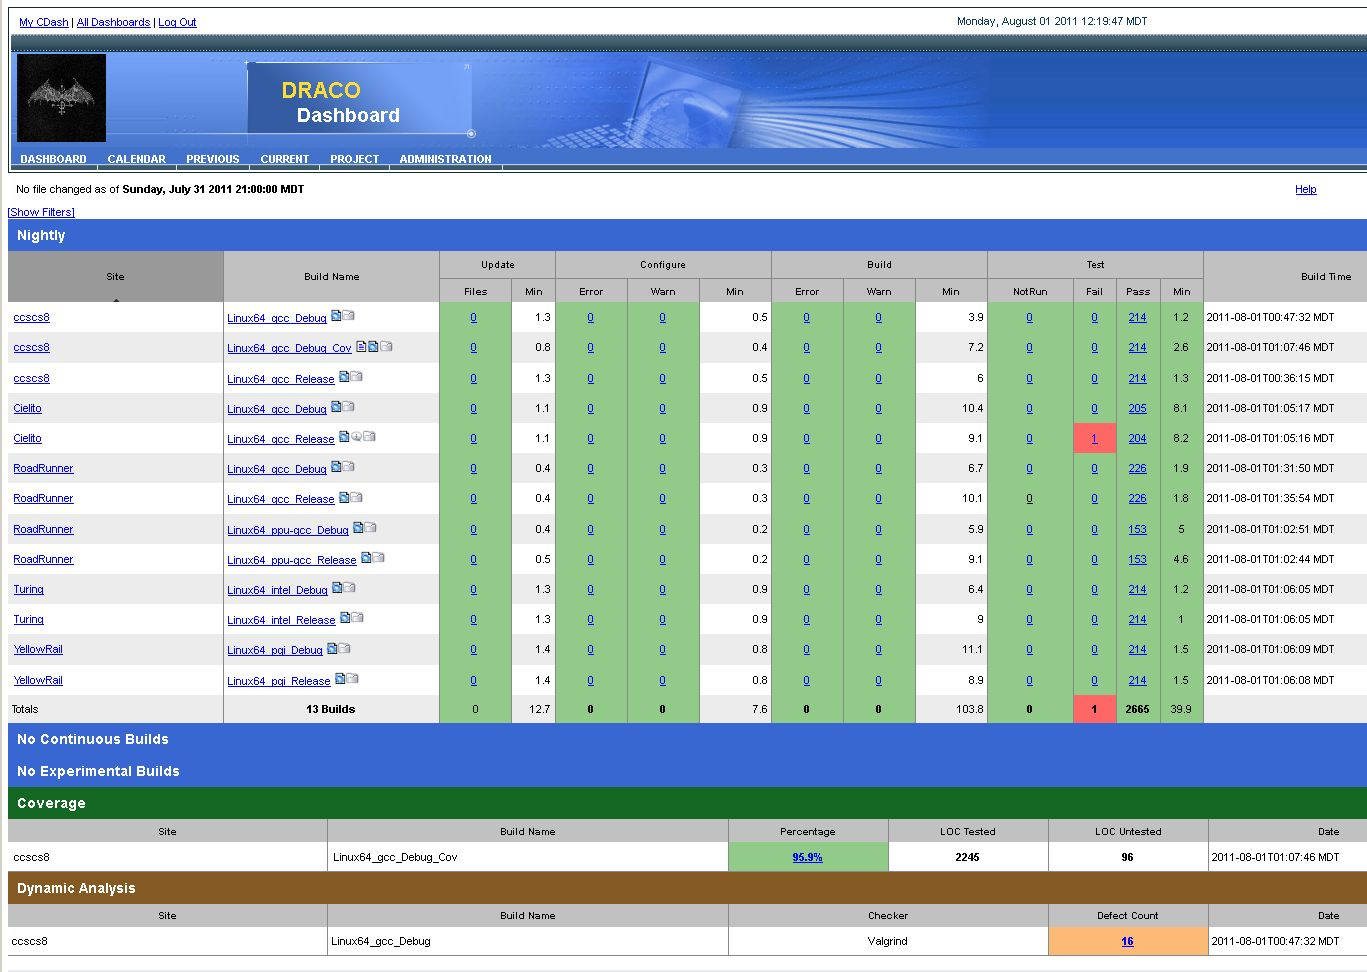
\includegraphics[width=8.0in,angle=90]{dashboard-620.jpg}}
  \caption{\cdash\ dashboard for \dracor\ hosted at \texttt{http://coder.lanl.gov.}}
\end{figure}
\begin{figure}
  \label{fig:ccdashboard}
  \centerline{
    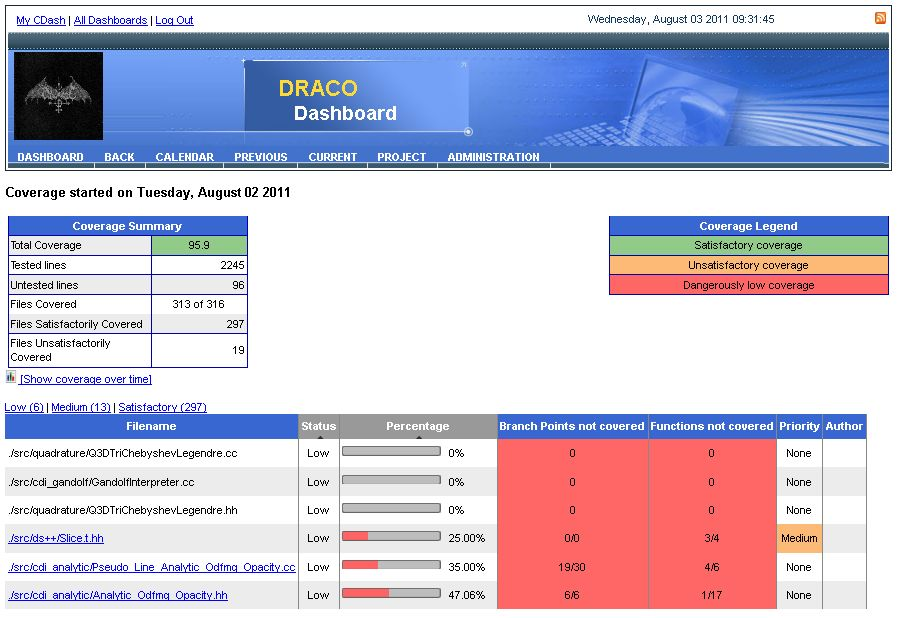
\includegraphics[width=6.0in,angle=0]{dashboard-cc-620.jpg}}
  \caption{\cdash\ dashboard for \dracor\ showing code coverage results.}
\end{figure}
\begin{figure}
  \label{fig:vgdashboard}
  \centerline{
    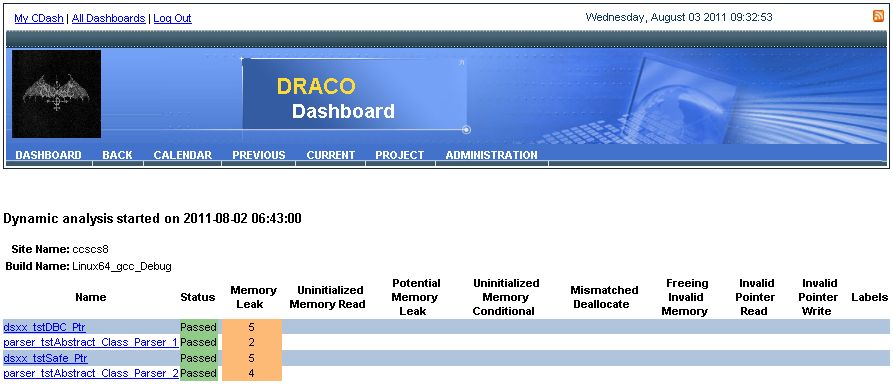
\includegraphics[width=6.0in,angle=0]{dashboard-valgrind-620.jpg}}
  \caption{\cdash\ dashboard for \dracor\ showing dynamic analysis results.}
\end{figure}
%%---------------------------------------------------------------------------%%

\section{Changes to individual components}
\label{sec:changes}
The following table summarizes changes to \draco\ components since
\draco-6\_0\_0. 

\subsection{General changes}
\label{changes:general}
\begin{itemize}

\item Component level release information and files have been
  eliminated from all components except \textsf{ds++}.  All other
  components will point to the general release information found in
  the \textsf{ds++} component.  \draco\ version numbers are now
  derived from the \cmake\ build system instead of being hard coded.
\item When using the \cmake\ GUI or \texttt{ccmake} some values are
  now contrained to permittable values (e.g.:
  \texttt{CMAKE\_BUILD\_TYPE}). 
\item Tweaks to test registration improve how tests are run in a
  threaded test environment (e.g.: \texttt{RESOURCE\_LOCK} to prevent
  tests from running at the same time, excluding some tests from
  valgrind analysis, etc.).
\item Cross-compiling support was added to support building \draco\ on
  Cielito and RoadRunner.

\end{itemize}

%% \subsection{meshReaders}
%% \label{changes:RTTFormatReader}
%% \begin{itemize}
%% \item Retire \texttt{Release.hh/cc} and point the code to
%%   \texttt{ds++/Release.hh/cc}.
%% \item Retire \scons\ scripts.
%% \end{itemize}

\subsection{c4}
\label{changes:c4}
\begin{itemize}
\item The \texttt{ApplicationUnitTest} class was redesigned so that it
  uses the CPP macro \texttt{DRACO\_UNAME} instead of the deprecated
  \texttt{C4\_UNAME}.  CPP macros of the form
  \texttt{c4\_is<platform>} are replaced with
  \texttt{draco\_is<platform>}. Finally, the define for
  \texttt{C4\_MPICMD} has been moved to \texttt{c4/config.h} and away
  from \texttt{ApplicationUnitTest.hh}.
\item \textsf{c4} now uses the new functions from
  \texttt{ds++/path.hh} instead of defining its own.
\item The \texttt{ApplicationUnitTest} class was updated so that it
  works on Cielito (i.e.: teach it to run \texttt{aprun}).
\item \texttt{C4\_Functions.hh} now defines a new function
  \texttt{send\_is} that will invoke \texttt{MPI\_Issend}.
\item \texttt{ParallelUnitTest} was updated to correct a deficiency
  that allowed the test to report \textsf{PASS} when a failure only
  occured on a non-IO processor.  A potential race condition found in
  the \texttt{status()} member function was removed.

\item \texttt{Send\_Receive} was updated so that the sender now holds
  onto size in a private member variable.  This prevents the value
  from going out of scope before the send completes.  \\
\\
  This change resolves the failure of the single-PE
  \textit{auto-communication test} in \texttt{tstSend\_Receive} on
  Cielito.  This test has typically passed on other machines, probably
  due to lucky buffering by MPI.  \texttt{MPI\_Isend} will not block
  waiting for a matching receive, but it's not required to buffer
  data.  The send buffer can only be safely reused (or destroyed, by
  any mechanism) after the send completes; i.e., after a Wait or Test.
\end{itemize}

\subsection{cdi}
\label{changes:cdi}
\begin{itemize}
\item In \texttt{OpacityCommon.hh}, a new enum value for
  \texttt{rtt\_cdi::Reaction} is provided to indicate the end of the
  enumeration list.  This is uselful for default initialization.
\end{itemize}

\subsection{cdi\_analytic}
\label{changes:cdi-analytic}
\begin{itemize}

\item Changed \texttt{Pseudo\_Line\_Analytic\_Opacity} to
  \texttt{Pseudo\_Line\_Analytic\_MultigroupOpacity}. This change
  supports implementing ODF opacities~\cite{ccs2:08-52} and pseudo
  line opacities in \textsf{Serrano}.

\item Renamed \texttt{Analytic\_Multigroup\_Opacity} to
  \texttt{nGray\_Analytic\_MultigroupOpacity}. This change supports
  implementing ODF opacities and pseudo line opacities in
  \textsf{Serrano}.

\item This component now depends on the \textsf{parser} and
  \textsf{ode} components, moving it from level 3 to level 4 in the
  levelization diagram as shown in Figure~\ref{fig:level}.
\end{itemize}

\subsection{cdi\_gandolf}
\label{changes:cdi-gandolf}
\begin{itemize}

\item A new utility, \texttt{GandolfInterpreter}, is provided to read
  \textsf{IPCRESS} files and interactively provide information about
  its content~\cite{gandolf,tops}.  An example use command is:
%
\begin{lstlisting}[basicstyle=\footnotesize,
    xleftmargin=1.0in, xrightmargin=1.0in]
% ./GandolfInterpreter file.ipcress
\end{lstlisting}
%
You can follow the prompts to query various parts of the IPCRESS file.
\item \texttt{GandolfWrapper} was modified to change the maximum
  allowed materials per file from 10 to 128.
\end{itemize}

\subsection{device}
\label{changes:device}
\begin{itemize}
\item This component is new for \dracor.  Its purpose is to provide an
  interface/handle for a heterogeneous computing device.  Currently,
  it wraps the DACS interface for RoadRunner.  In the future it may
  also provide an interface to GPUs or special threading models.
\item Currently, this component is only available when building on
  RoadRunner. 
\item \texttt{DACS\_Device} is a singleton for DACS host-side resource
  and process management. 
\item \texttt{DACS\_Process} is an abstract host-side representation of
  an accel-side process.  \texttt{DACS\_Process} represents an
  accel-side process.  It provides methods to start and stop the
  accel-side process, and accessors that return the filename of the
  accel-side binary and the pid of the running process.  Clients
  should inherit from \texttt{DACS\_Process} and implement the stop
  method.  
\end{itemize}

%% \subsection{diagnostics}
%% \label{changes:diagnostics}
%% \begin{itemize}
%% \item Retire \texttt{Release.hh/cc} and point the code to
%%   \texttt{ds++/Release.hh/cc}.
%% \item Retire \scons\ scripts.
%% \end{itemize}

%% %% The \textsf{diagnostics} component is new for \dracor.  This component
%% %% was moved to \draco\ from \textsc{clubimc} where it was known as
%% %% \textsf{utils}.  This transition was made because this is a generic
%% %% component (not specific to \textsc{clubimc} or \textsc{Jayenne}) and
%% %% because the library name was conflicting with a \textsc{Capsaicin}
%% %% component that was also named \textsf{utils}.

%% %% This component provides a CPP macro that controls code verbosity.
%% %% There are two new configure commands that enable the diagnostics
%% %% (i.e.: verbosity) level:
%% %% %
%% %% \begin{center}
%% %%   \footnotesize
%% %%   \begin{tabular}{lp{4.0in}}
%% %%     \hline\hline

%% %%     \texttt{--with-draco-diagnostics=[0-7]} & \tableText{When greater
%% %%       than zero, the CPP macro \texttt{DRACO\_DIAGNOSTICS} is set to
%% %%       the provided value.} \\

%% %%     \texttt{--with-draco-timing=[0-2]} & \tableText{When greater than
%% %%       zero, the CPP macro \texttt{DRACO\_TIMING} is set to 2.} \\
 
%% %%     \hline\hline 
%% %%   \end{tabular}
%% %% \end{center}
%% %% %
%% %% These CPP macros are saved to the \texttt{config.h} for the
%% %% \textsf{diagnostics} component.  The values are designed to take the
%% %% form of a bit mask in a method identical to what is used for \draco's
%% %% DbC feature.
%% %% %
%% %% \begin{center}
%% %%   \footnotesize
%% %%   \begin{tabular}{llp{4.0in}}
%% %%     \hline\hline
%% %%     \textbf{value} & \textbf{bit mask} & \textbf{description} \\
%% %%     \hline
%% %%     0 & 000 & \tableText{Extra verbosity disabled.} \\
%% %%     1 & 001 & \tableText{Sets CPP macro \texttt{DRACO\_DIAGNOSTICS\_LEVEL\_1}.} \\
%% %%     2 & 010 & \tableText{Sets CPP macro \texttt{DRACO\_DIAGNOSTICS\_LEVEL\_2}.} \\
%% %%     4 & 100 & \tableText{Sets CPP macro \texttt{DRACO\_DIAGNOSTICS\_LEVEL\_3}.} \\

%% %%     \hline\hline 
%% %%   \end{tabular}
%% %% \end{center}

%% %% Here is an example of how the \textsf{diagnostic} feature is used by
%% %% \textsc{Jayenne}.

%% %% \lstset{language=C++,
%% %%   showstringspaces=false,
%% %%   frame=shadowbox,
%% %%   basicstyle=\footnotesize,
%% %%   rulesepcolor=\color{black},
%% %%   backgroundcolor=\color{listingBG}
%% %% }
%% %% \begin{lstlisting}[xleftmargin=0.50in, xrightmargin=0.50in]
%% %% #ifdef DRACO_DIAGOSTICS_LEVEL_1
%% %% {
%% %%      using namespace rtt_diagnostics::Diagnostics;
%% %%      int local_end_census       = integers["End_census"];
%% %%      rtt_c4::global_sum(local_end_census);
%% %%      if (ncentot != local_end_census)       ITFAILS;
%% %% }
%% %% #endif
%% %% \end{lstlisting}

%% %% The timing diagnostic is used by
%% %% \texttt{wedgehog\_managers/Diagnostics\_Output.hh}.  An excerpt is
%% %% shown here: 
%% %% \begin{lstlisting}[xleftmargin=0.50in, xrightmargin=0.50in]
%% %% #ifdef DRACO_TIMING_ON
%% %%     {
%% %%         // print out a timing table

%% %%         // get the keys
%% %%         Timing_Diagnostics::Vec_Keys keys = Timing_Diagnostics::timer_keys();
%% %%         int Nk                            = keys.size();

%% %%         // determine max/min
%% %%         vector<double> max(keys.size(), 0.0);
%% %%         vector<double> min(keys.size(), 0.0);

%% %%         double v = 0.0;
%% %%         for (int i = 0; i < Nk; ++i)
%% %%         {
%% %%             // get the value of the timer
%% %%             v = Timing_Diagnostics::timer_value(keys[i]);

%% %%             // get the local value
%% %%             max[i] = v;
%% %%             min[i] = v;
%% %%         }

%% %%         // get the max/min value across all processors
%% %%         rtt_c4::global_min(&min[0], Nk);
%% %%         rtt_c4::global_max(&max[0], Nk);

%% %%         rtt_c4::global_barrier();
%% %%         if (rtt_c4::node() == 0)
%% %%         {
%% %%             // output the max/mins
%% %%             cout << setw(25) << "Routine" << setw(15) << "Max Fraction"
%% %%                  << setw(15) << "Min Fraction" << endl;
%% %%             cout << "======================================================="
%% %%                  << endl;
%% %%             for (int i = 0; i < Nk; ++i)
%% %%             {
%% %%               if (cycle_tot != 0.0)
%% %%               {
%% %%                   cout << setw(25) << keys[i] << setw(15) << max[i] / cycle_tot
%% %%                        << setw(15) << min[i] / cycle_tot << endl;
%% %%               }
%% %%               else
%% %%               {
%% %%                 cout << "WARNING: Time to complete cycle is ZERO seconds!"
%% %%                      << endl;
%% %%               }
%% %%             }
%% %%             cout << "======================================================="
%% %%                  << endl;
%% %%         }
%% %%         rtt_c4::global_barrier();

%% %%         // reset the timers
%% %%         Timing_Diagnostics::reset_timers();
%% %%     }
%% %% #endif
%% %% \end{lstlisting}
%% %% \lstset{language=ksh,
%% %%   showstringspaces=false,
%% %%   frame=shadowbox,
%% %%   basicstyle=\footnotesize,
%% %%   rulesepcolor=\color{black},
%% %%   backgroundcolor=\color{listingBG}
%% %% }

\subsection{ds++}
\label{changes:dsxx}
\begin{itemize}
\item The \texttt{Allocators} class was retired.\\ 
     In practice, this class was designed before the STL allocators
     class was finalized and was deficient when compared to current
     standards.  There are other design defects that caused repeated
     compiler warnings. Also, the Allocators classes were only being
     used by \texttt{ds++/Mat.hh} and this class was designed so that
     only the \texttt{Simple\_Allocator} would work. It was impossible
     to instantiate \texttt{Mat[1-5]} with the
     \texttt{Guarded\_Allocator<T>}.  The plan is to update
     \texttt{Mat.hh} to use \texttt{std::allocators<T>}.  This still
     allows more sophisticated allocators to be used in the future and
     allow us to eliminate \texttt{ds++/Allocators.hh}.
\item The \texttt{DynArray} class was retired.
\item \texttt{Mat} classes were updated to use STL allocators instead
  of \texttt{ds++/Allocators}, which are being retired.
\item A new function \texttt{verbose\_error()} in \texttt{path.hh} is
  provided.
\item \texttt{UnitTest} was refactored by moving some file/path
  manipulation logic into \texttt{ds++/path.hh}.
\item \texttt{path} was updated by providing the member functions
  \texttt{fileExists()} and \texttt{getFilenameComponent()}.
\item \texttt{swap.hh} was added.  This class provides functions that
  do byte-swapping in one of two ways: either use GNU extended asm for
  x86 (really f86+), or use the \textit{poor people's} method of
  digging out one byte at a time and moving it to the right place.
  The poor method is really not that bad: GCC for example seems to
  optimize it down to about 5 instructions in the 32 bit case,
  including loads, versus 2 instructions (including load) for the
  inline asm case.
\item Establish \texttt{Release.hh/cc} as the Release information for
  all \draco\ componenets.
\end{itemize}

%% \subsection{fit}
%% \label{changes:fit}
%% \begin{itemize}
%% \item
%% \item Establish \texttt{Release.hh/cc} as the Release information for
%%   all \draco\ componenets.
%% \item Retire \scons\ scripts.
%% \end{itemize}

%% \subsection{fpe\_trap}
%% \label{change:fpe-trap}
%% \begin{itemize}
%% %% \item The functionality of this package was inadvertantly disabled on
%% %%   Linux64 due to an autoconf script defect.  The package has been
%% %%   reactivated.
%% %% \item On Darwin, it appears that the SIGFPE is caught, but the
%% %%   operating system still aborts the process and pops up a GUI
%% %%   information box to this effect.  There is no clear path forward to
%% %%   fix this problem.
%% %% \item New package in \draco-5\_9\_0.
%% %% \item Remove dependency on \textsf{c4}.
%% \end{itemize}

\subsection{lapack\_wrap}
\label{changes:lapackwrap}
\begin{itemize}
\item The build system will now omit \texttt{lapack\_wrap} from the build
  if \textsf{LAPACK} is not found.
\end{itemize}

\subsection{linear}
\label{changes:linear}
\begin{itemize}
\item \texttt{ludcmp.i.hh} was modified to use \texttt{abs} from
  \textsf{ds++} instead of \texttt{cstdlib.h}. The dsxx version
  provides specialization for \texttt{double} and eliminates a gcc
  warning when compiling on rr-dev.
\item This component does not depend on \textsf{traits}, so remove this
  linkage from \texttt{CMakeLists.txt}.
\end{itemize}

%% \subsection{meshReaders}
%% \label{changes:meshreaders}
%% \begin{itemize}
%% \item
%% \item Retire \texttt{Release.hh/cc} and point the code to
%%   \texttt{ds++/Release.hh/cc}.  
%% \item Retire \scons\ scripts.
%% \end{itemize}

%% \subsection{mesh\_element}
%% \label{changes:mesh-element}
%% \begin{itemize}
%% %% \item Added generic element identifier and support.
%% \end{itemize}

%% \subsection{min}
%% \label{changes:min}
%% \begin{itemize}
%% %% \item Added generic element identifier and support.
%% \end{itemize}
%% \subsection{parser}

%% \subsection{norms}
%% \label{changes:norms}
%% \begin{itemize}
%% %% \item Added generic element identifier and support.
%% \end{itemize}
%% \subsection{parser}

%% \subsection{ode}
%% \label{changes:ode}
%% \begin{itemize}
%% %% \item Added generic element identifier and support.
%% \end{itemize}
%% \subsection{parser}

\subsection{parser}
\label{changes:parser}
\begin{itemize}
\item Expanded initialization syntax for \texttt{Expression} to allow
  general expressions.
\end{itemize}

\subsection{quadrature}
\label{changes:quadrature}
\begin{itemize}

\item In \texttt{Angle\_Operator}, added a capability to choose to add
  an additional set of starting directions which are zero-weight,
  outwardly directed angles on a level that are opposite the inwardly
  directed angles usually used for the starting direction calculation
  in curvilinear coordinates. \\
  The \textit{enforce exact symmetry} flag for the sweeper is now a
  bool and is set to be \texttt{false} by default. This change
  requires that many of the application test input files be modified
  to turn this flat on because the base files were calculated with the
  previous default of being turned on.

\item In \texttt{Angle\_Operator}, added a \texttt{vector<unsigned>}
  data member and accessor that contains the angle index into the
  most-positive outwardly directed angle on every level for ordinate
  sets constructed for curvilinear coordinates.  These are the angles
  used to reflect the starting direction angular fluxes.

\item \texttt{Ordinate} was updated so that the ordinates can be
  sorted based on a comparator supplied to the \texttt{QuadServices}
  constructor.  Also fixed an inconsistency in ordering of
  ordinates. Fix incorrect multiplication of source by opacity. Now
  returns constant solution for $S_6$ and source boundaries.

\item Added support for \textit{3D triangular Chebyshev} quadrature.

\item In \texttt{QuadServices}, add a missing
  \texttt{gsl\_permutation\_free}, to match
  \texttt{gsl\_permutation\_alloc}. This eliminates the five memory
  leaks reported by \textsf{valgrind}. 
\end{itemize}

%% \subsection{rng}
%% \label{changes:rng}
%% \begin{itemize}
%% %% \item Added some convenient pseudo-random number generators:
%% %%   \textsf{Halton\_Sequence}, \textsf{Halton\_Subrandom\_Generator},
%% %%   \textsf{Sobol\_Sequency} and \textsf{LC\_Subrandom\_Generator}.
%% %% \item Extracted, rewrote and implemented parts of the SPRNG library to
%% %%   provide a more efficient inline random number stream.
%% %% \item Extended unit tests to provide better function point coverage.
%% %% \item Commented out unused functions and function arguments as
%% %%   identified by g++.
%% \end{itemize}

%% \subsection{roots}
%% \label{changes:roots}
%% \begin{itemize}
%% %% \item
%% \end{itemize}

\subsection{special\_functions}
\label{changes:special-functions}
\begin{itemize}

\item Added an exponential integral evaluation function,
  \texttt{ExpInt}. This routine is extracted from
  from~\cite{numericalrecipesforcpp}.  It computes the general
  exponential integrals of type $Ei(x)$ or $E_n(x)$. \\
  \\
  $E_n(x)$ is calculated either by special case definitions for $n=0$
  or $x=0$ with $n=0$ or $1$, or the Lentz algorithm if $x>1.0$, or
  the digamma series representation for greater $x$. \\
  \\
  $Ei(x)$ is calculated using power series expansion for
  $x<|ln(EPS)|$, where $EPS$ is the required relative error (set to
  machine precision), as this is the lower limit of the asymptotic
  series, which is used for greater values of $x$. The asymptotic
  series includes all converging terms until values are less than
  $EPS$. $Ei(-x)$ evaluates to the extension $-E_1(x)$.
\end{itemize}

\subsection{timestep}
\label{changes:timestep}
\begin{itemize}
\item Refactored some code and the unit tests to improve code
  coverage.  In particular, capture some of the output that was going
  to \texttt{cout} and examine it from within the tests.
\end{itemize}

\subsection{traits}
\label{changes:traits}
\begin{itemize}
\item Retire \texttt{Release.hh/cc} and point the code to
  \texttt{ds++/Release.hh/cc}.  
\item With the above change, this component is now a header only
  package.  No library will be built or installed.
\end{itemize}

%% \subsection{units}
%% \label{changes:units}
%% \begin{itemize}
%% %% \item Added {\it cgsh} and {\it cgmu} unit systems.
%% %% \item Added output unit system specification.
%% \end{itemize}

%% \subsection{viz}
%% \label{changes:units}
%% \begin{itemize}
%% %% \item Added unit tests to bring the function point code coverage above
%% %%   80\%.
%% %% \item Update code base to make correct use of signed vs. unsigned
%% %%   integer types.
%% %% \item Wrap OS specific command (e.g.: \texttt{mkdir} or \texttt{rm})
%% %%   as CPP macros defined in \texttt{config.h}.
%% \end{itemize}
%% %------------------------------------------------------------------------------%

\section{Defects}

Known defects are listed on LANL's TeamForge web server
(\url{tf.lanl.gov}).  Here is a list of known defects:
\begin{itemize}
\item \texttt{cdi\_gandolf} will crash with a segmentation violation
  if a bad key is provided.
\item \texttt{c4/tstComm\_Dup} fails for optimized builds on Cielito.
\end{itemize}

\noindent Here is a list of defects corrected in this release.
\begin{itemize}
\item Bugs associated with RedStorm and Purple are closed because those machines
  have been retired. See
  \href{https://tf.lanl.gov/sf/sfmain/do/go/artf6975}{artf6975} and
  \href{https://tf.lanl.gov/sf/sfmain/do/go/artf9622}{artf9622}. 
\item Bugs associated with the autoconf-based build system are
  closed because that build system is now deprecated. See
  \href{https://tf.lanl.gov/sf/sfmain/do/go/artf1860}{artf1860},
  \href{https://tf.lanl.gov/sf/sfmain/do/go/artf1852}{artf1852},
  \href{https://tf.lanl.gov/sf/sfmain/do/go/artf6894}{artf6894},
  \href{https://tf.lanl.gov/sf/sfmain/do/go/artf5895}{artf5895},
  \href{https://tf.lanl.gov/sf/sfmain/do/go/artf3896}{artf3896}, and
  \href{https://tf.lanl.gov/sf/sfmain/do/go/artf1876}{artf1876}.
\item \href{https://tf.lanl.gov/sf/sfmain/do/go/artf20373}{artf20373}
  is closed by retiring the \texttt{Allocators} feature.
\item \href{https://tf.lanl.gov/sf/sfmain/do/go/artf20019}{artf20019}
  is closed by consolidating all \texttt{Release} files into a single
  file that is now in ds++.
\item '\href{https://tf.lanl.gov/sf/sfmain/do/go/artf20183}{CDash
  shows a different number of files updated}' has been fixed/closed.
\item The parser package has been updated and now compiles with the
  PGI compiler set. See
  \href{https://tf.lanl.gov/sf/sfmain/do/go/artf4652}{artf4652}.
\item All active components now have good unit test code coverage. See
  \href{https://tf.lanl.gov/sf/sfmain/do/go/artf1877}{artf1877}. 
\end{itemize}

%------------------------------------------------------------------------------%

\section{Design}

There are no inter/intra-component cyclic dependencies in \draco.  The
levelized graph for \dracor\ components is shown in
Fig.~\ref{fig:level}.  The diagram includes the one new package,
\textsf{device} and shows the new dependency on \textsf{parser} for
\textsf{cdi\_analytic}. The new dependency pushes
\textsf{cdi\_analytic} into Level~4.

\draco\ requires a few vendor libraries.  These include the
\textsf{GNU Scientific Library}~\cite{gslref}, \textsf{Message Passing
  Interface (MPI)}~\cite{openmpiweb} and
\textsf{LAPACK}~\cite{lapackweb}.  Additional functionality is
provided by \draco\ if the following vendors are available:
\textsf{GANDOLF}~\cite{gandolf}, \textsf{dlopen} and
\textsf{XMGRACE}~\cite{xmgraceweb}.

\begin{figure}
  \label{fig:level}
  \centerline{
    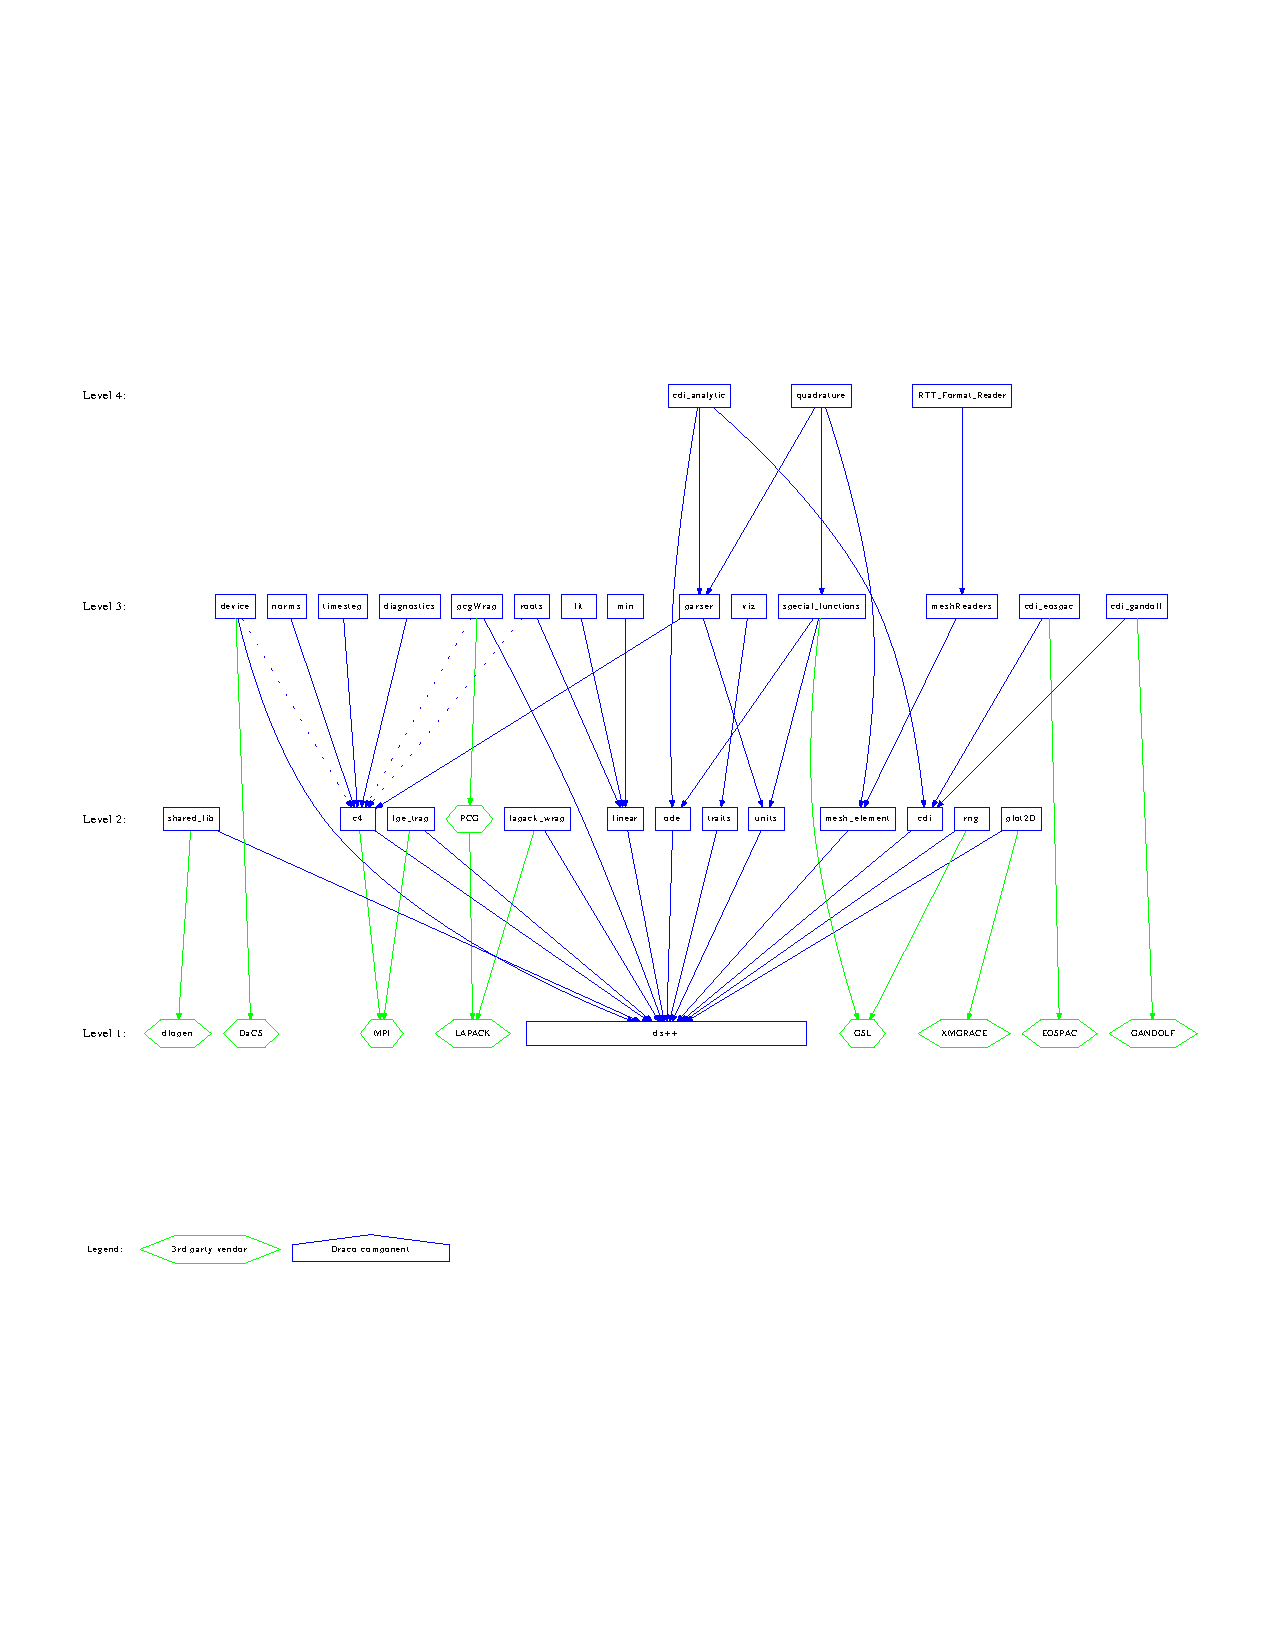
\includegraphics[width=8.5in,angle=90]{level-6_2_0.pdf}}
  \caption{\dracor\ levelized component graph.  Dotted lines signify
    that the dependency is only required for testing.}
\end{figure}

%------------------------------------------------------------------------------%

\section{Code Statistics}

%% http://cloc.sourceforge.net v 1.54  T=24.0 s (74.3 files/s, 11525.5 lines/s)
%% --------------------------------------------------------------------------------
%% Language                      files          blank        comment           code
%% --------------------------------------------------------------------------------
%% C++                             422          14847          21712          72047
%% Text                            174           5938           5237          44318
%% C/C++ Header                    364           8516          23485          21544
%% Lisp                             12           1218           1831           6655
%% m4                               50           2042           2471           5876
%% CMake                            98           1655           3732           5241
%% Bourne Shell                     22            486           1081           4039
%% Python                           39           1777           1922           3184
%% XML                               9           1085              0           2798
%% CVS                             501             19              0           2706
%% make                             52            905            975           1855
%% Perl                              1            690            106           1828
%% C                                32            390            811            750
%% CSS                               1            113             37            395
%% C Shell                           2             17             23             67
%% Bourne Again Shell                1              7             24             55
%% HTML                              2              8             15             45
%% awk                               1              6              2             27
%% --------------------------------------------------------------------------------
%% SUM:                           1783          39719          63464         173430
%% --------------------------------------------------------------------------------

% tools/count_loc.sh 

%% Counting lines of source code -- 
%% Directory:  /home/kgt/draco
%% Date     :  Tue Aug 2 09:15:02 MDT 2011

%%                  Total C++ source: 40006
%%    C++ source in test directories: 22481
%%       C++ contract specifications: 1494
%%                      C++ comments: 42763
%%              Total Fortran source: 12
%%                  Fortran comments: 4
%%               LaTeX Documentation: 16045
%%                       HTML source: 0
%%                         Text docs: 6768
%%        Build system script source: 111510
%%    Executable shell script source: 3239
%%            Executable Perl source: 1867
%%                     Python source: 3906
%%                     Expect source: 0
%%                      Elisp source: 6695

%% Done.


Lines-of-Code (LOC) statistics for all \draco\ releases are are shown
in Fig.~\ref{fig:stats}.  The large drop between \draco-4\_0\_0 and
\draco-5\_0\_0 is due to the removal of the \textsf{mc} and
\textsf{imc} packages. The aggregate LOC statistics for \dracor\ are:
\begin{center}
  \begin{tabular}{|l|r|} \hline
    Total component package source code & 40006 \\
    Total unit test code & 22481 \\
    Total DBC statements & 1494 \\
    Total comments & 42763 \\
    \hline
  \end{tabular}
\end{center}

\begin{figure}
  \label{fig:stats}
  \centerline{
    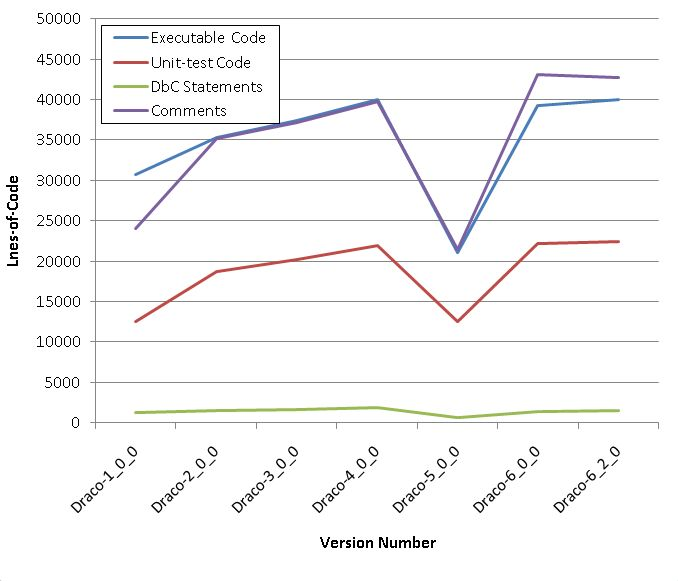
\includegraphics[width=4.5in]{loc-6_2_0.jpg}}
  \caption{LOC statistics for \dracor\ component packages.}
\end{figure}

%% Table~\ref{tab:loc} shows LOC metrics for each \draco\ component in
%% \dracor.  LOC metrics are stored in \draco\ in
%% \texttt{draco/doc/code\_stats}.
%% \begin{table}
%%   \caption{
%%     LOC metrics for component packages in \dracor.  DBC LOC refers to
%%     Design-by-Contract$^{\copyright}$ statements. 
%%   }
%%   \label{tab:loc}
%%   \begin{center}
%%     \begin{tabular}{lrrr}\hline\hline
%%       \multicolumn{1}{c}{Component} &
%%       \multicolumn{1}{c}{Source LOC} &
%%       \multicolumn{1}{c}{DBC LOC} &
%%       \multicolumn{1}{c}{Test LOC} \\\hline
%%       RTT\_Format\_Reader &     2408     &       19      &      1063     \\
%%       c4                 &      2702     &       86      &      1294     \\
%%       cdi                &      1566     &       82      &      1122     \\
%%       cdi\_analytic      &      1436     &      110      &       771     \\
%%       cdi\_gandolf       &      2150     &       45      &      1248     \\
%%       diagnostics        &       333     &        4      &       267     \\
%%       ds++               &     11155     &      337      &      8147     \\
%%       fit                &        95     &        3      &        56     \\
%%       fpe\_trap          &       117     &        5      &        51     \\
%%       lapack\_wrap       &       193     &       37      &       116     \\
%%       linear             &      1083     &       51      &       462     \\
%%       meshReaders        &       454     &       16      &       261     \\
%%       mesh\_element      &      1270     &       36      &       727     \\
%%       min                &       631     &        2      &       399     \\
%%       norms              &       282     &        4      &       160     \\
%%       ode                &       193     &        6      &        86     \\
%%       parser             &      3182     &      218      &      1475     \\
%%       plot2D             &       329     &       30      &        76     \\
%%       quadrature         &      3106     &      192      &      1195     \\
%%       rng                &       355     &       18      &       184     \\
%%       roots              &       670     &        8      &       219     \\
%%       shared\_lib        &       184     &       12      &       118     \\
%%       special\_functions &       976     &       10      &       490     \\
%%       timestep           &       533     &       16      &       196     \\
%%       traits             &       134     &       9       &       47      \\
%%       units              &      1401     &       11      &       1186    \\
%%       viz                &       680     &       47      &       209     \\
%%       xm                 &       414     &       4       &       257     \\
%%       \hline\hline
%%     \end{tabular}
%%   \end{center}
%% \end{table}

%% %% cd draco/src
%% %% for dir in `/bin/ls -1 -d */`; do echo "---- $dir ----''; (cd $dir;\
%% %% ../../tools/count_loc.sh); done 

With the adoption of the \textsf{Bullseye}~\cite{bullseyeweb} coverage
analysis tool, we are better able to track unit-test coverage of
\draco\ components.  The goal is to achieve 100\% functional test
coverage for each \draco\ component.  Table~\ref{tab:coverage} gives
functional and conditional point coverage for \dracor.  This table
shows a slight improvement in the function point coverage
(approximately 2\% improvement) when compared to \draco-6\_0\_0.
%%---------------------------------------------------------------------------%%
%% coverage table for draco-6_0_0
%%---------------------------------------------------------------------------%%

%% export COVFILE=/home/regress/cmake_draco/Nightly_gcc/Coverage/build/CMake.cov
%% export COVDIRCFG=/home/regress/cmake_draco/Nightly_gcc/Coverage/build/covclass_cmake.cfg
%% cd /home/regress/cmake_draco/Nightly_gcc/Coverage/source/src
%% covdir 

\begin{table}
  \caption{
    Unit-test coverage in \dracor.  C/D Coverage refers to conditional
    statements.  We strive for 100\% function point coverage.  
  }
  \label{tab:coverage}
  \begin{center}
    \begin{tabular}{lcrcr}\hline\hline
      \multicolumn{1}{c}{Component} &
      \multicolumn{1}{c}{Function Coverage} &
      \multicolumn{1}{c}{Percent (\%)} &
      \multicolumn{1}{c}{C/D Coverage} &
      \multicolumn{1}{c}{Percent (\%)} \\\hline

viz/                 &   24 /    25 &  96 &    129 /   168 &  76  \\
units/               &   82 /    82 & 100 &     58 /    58 & 100 \\
traits/              &   16 /    16 & 100 &      0 /     0        \\
timestep/            &   59 /    62 &  95 &    104 /   178 &  58 \\
special\_functions/  &   29 /    29 & 100 &    190 /   198 &  95 \\
roots/               &    8 /     8 & 100 &    256 /   312 &  82 \\
rng/                 &   62 /    67 &  92 &     63 /    70 &  90 \\
quadrature/          &  167 /   182 &  91 &    517 /   631 &  81 \\
parser/              &  246 /   266 &  92 &   1050 /  1351 &  77 \\
ode/                 &    5 /     5 & 100 &     29 /    32 &  90 \\
norms/               &   25 /    26 &  96 &     21 /    34 &  61 \\
min/                 &    9 /     9 & 100 &    137 /   154 &  88 \\
mesh\_element/       &    24 /    24 & 100&     165 /   213 &  77 \\
meshReaders/         &   15 /    15 & 100 &    127 /   172 &  73 \\
linear/              &   16 /    16 & 100 &    324 /   392 &  82 \\
lapack\_wrap/        &    11 /    16 &  68&       0 /     0        \\
fpe\_trap/           &     2 /     2 & 100&       4 /    11 &  36 \\
fit/                 &    1 /     1 & 100 &     15 /    16 &  93 \\
ds++/                &  654 /   673 &  97 &    602 /   679 &  88 \\
diagnostics/         &    8 /     8 & 100 &      4 /     4 & 100 \\
cdi\_gandolf/        &   129 /   132 &  97&     154 /   278 &  55 \\
cdi\_analytic/       &   130 /   143 &  90&     156 /   200 &  78 \\
cdi/                 &   39 /    39 & 100 &     27 /    30 &  90 \\
c4/                  &  169 /   174 &  97 &    288 /   338 &  85 \\
RTT\_Format\_Reader/ &    315 /   321 &  9&8     273 /   356 &  76 \\

     \hline
      {\bf Total} & {\bf 2245/2341} & {\bf 95} & {\bf 4693/5875} & {\bf 79} \\

      \hline\hline
    \end{tabular}
  \end{center}
\end{table}

%%---------------------------------------------------------------------------%%
%% end of coverage table
%%---------------------------------------------------------------------------%%


The \cdash\ \hyperref[http://coder.lanl.gov/cdash]{dashboard} for
\draco\ presents all of these code statistics and also valgrind
results for nightly regression builds.  The data is presented in a
more interactive format that is more useful for day-to-day
development.

%% %%---------------------------------------------------------------------------%%

%% \section{\draco\ Build System}
%% \label{sec:dbs}

%% The traditional autoconf-based \draco\ Build System (DBS) has
%% undergone some significant changes.  The most significant changes are
%% support for new platforms and compiler sets, new vendor libraries and
%% more automation.  The build system required the developer to provide
%% fewer command line arguments and will choose reasonable defaults in
%% most cases.  Ultimately, the developer still has the ability to avoid
%% using any default value by specifying his or her own options on the
%% configure line.  Specific changes to the build system are itemized
%% here: 
%% \begin{itemize}
%% \item Separated the build and testing phases in the
%%   \texttt{Makefiles}.  This change is needed becuase of limitations on
%%   ASC hardware where we build on the front end but run the tests on
%%   the worker nodes.  \texttt{make} alone will build the libraries.
%%   \texttt{make all} will build all libraries and unit tests, but not
%%   run them.   \texttt{make check} will compile all libraries and unit
%%   tests and run all unit tests.  \texttt{make run} will run the tests
%%   without trying to build anything.
%% \item Provided support for building a stubbed out version of
%%   \textsf{cdi\_gandolf}.
%% \item Changed the build system so that it tries to determine if either
%%   \texttt{-lgfortran} or \texttt{-lg2c} are needed on the link lines.
%% \item No longer store generated \texttt{aclocal.m4} files in \CVS.
%% \item Support for STLPort cleaned up in \draco-5\_5\_0.
%% \item Simplified autoconf-based build system to eliminate the
%%   requirement for lengthy configure commands.  Most options are now
%%   defaulted to reasonable values.
%% \item Added support for Intel compilers (icc, icpc, ifort).
%% \item Added support for RoadRunner's PPE cross compiler, ppu-g++.
%% \item Added support for gcc-4+ including gfortran.
%% \item Improved support for IBM xlc compiler and AIX.
%% \item Improved support for PGI compilers (pgcc, pgCC, pgfort)
%% \item Added support for linking FORTRAN main programs.
%% \item Added support for new vendors including Silo, ParMetis, NDI and
%%   SuperLU\_DIST.
%% \item Added unofficial support for Darwin (PPC and Intel) and MSVC on
%%   Windows (note that not all packages can be compiled on these
%%   architectures).
%% \item Many \texttt{config.h.in} files were modified to support
%%   configuration with either \textsf{autoconf} or \textsf{CMake}. A new
%%   define for \texttt{AUTOCONF} is found in both \texttt{configure.ac}
%%   files and in \texttt{config.h.in} to keep the 2 build systems
%%   working simultaneously.
%% \item Corrected a glitch in the config scripts that assumed that
%%   \texttt{CXX} would be the name of a comiler without the full path
%%   prepended.  On the HPC hardware or when using \draco\ modules, this
%%   variable always uses the full path to the compiler.
%% \end{itemize}

%% Additionally, a prototype \textsf{scons} build system was implemented
%% while porting Jayenne codes to RoadRunner.  While this build system
%% remains mostly intact, it is not being adopted or maintained for this
%% release. A prototype \textsf{CMake} build system has been added
%% recently and will be evaluated early in 2011 to determine if
%% \draco\ development will move to the CMake-based system.  The
%% CMake-based system required less scripting code to be supported by the
%% \draco\ team, it has better dependency checking, better parallel build
%% support, a mature testing system and suppport for dashboard reporting.
%% The current prototype reports results to \url{coder.lanl.gov/cdash}.

%% Two new top-level configure options have been added to the build
%% system.  The first turns up the warning level for \gpp\ and the second
%% provide additional checks (similar to STLPort) at run time.  The new
%% options are detailed below:
%% %
%% \begin{center}
%%   \footnotesize
%%   \begin{tabular}{lp{4.0in}}
%%     \hline\hline
%% \texttt{--enable-all-warnings} & 
%%      \tableText{For g++, this option turns on -Wall and -Wextra.
%%        \draco\ was updated to build cleanly with theses flags, but
%%        they are not the default yet.} \\ 
%% \texttt{--enalbe-glibcxx-debug} &
%%      \tableText{For g++, this option uses the debug GLIBCXX
%%        libraries.  This option provides bounds checking for STL
%%        containers and more.  It addes the following defines to
%%        \texttt{CXXFLAGS}: \texttt{-D\_GLIBCXX\_DEBUG
%%          -D\_GLIBCXX\_DEBUG\_PEDANTIC}. } \\
%%     \hline\hline
%%   \end{tabular}
%% \end{center}

%% It is no longer required to use configure options like
%% \texttt{--with-mpi-inc --with-mpi-lib}.  The build system will set
%% these values automatically if your environment is set correctly. (It
%% will be if you use the environment/Modules!)  That is, you will need
%% to set \texttt{MPI\_INC\_DIR} and \texttt{MPI\_LIB\_DIR} in your
%% environment before running configure.  If MPI is not found in your
%% environment, the build system will automatically default to the
%% \texttt{--with-c4=scalar} option.  This trend will hold true for other
%% vendor libraries as well (GSL, Trilinos, LAPACK, etc.).  If a vendor
%% library is not found, then dependent \draco\ components will be
%% omitted.  For example, if GSL is not found by the build system then
%% \textsf{quadrature}, \textsf{rng} and \textsf{special\_functions} will
%% not be built.

%%---------------------------------------------------------------------------%%

\section{\draco\ Directory Structure}

The current \draco\ directory structure is shown below:
\begin{lstlisting}[basicstyle=\footnotesize, xleftmargin=2.0in, 
  xrightmargin=2.0in]
draco/
    src/
        ds++/
        c4/
        ...
    doc/
        gettingStarted/
        releases/
        ...
    tools/
    autodoc/
    config/
    environment/
        Modules/
        bashrc/
        bibfiles/
        bibtex/
        bin/
        elisp/
        latex/
        python/
        share/
        templates/
\end{lstlisting}
Table~\ref{tab:envdir} describes the purpose of each of the
\texttt{environment} directories in detail.  The rest of the
\draco\ directory structure is self-explanitory.
\begin{table}[!ht]
  \caption{
    Descriptions of the directories in \texttt{draco/environment}.
    The \draco\ development environment is entirely encapsulated
    within the \texttt{environment} directory.
  }
  \label{tab:envdir}
  \begin{center}
    \begin{tabular}{lp{3in}}\hline\hline
      \multicolumn{1}{c}{Directory} & 
      \multicolumn{1}{c}{Description} \\ \hline
      
      \texttt{Modules} & \tableText{initialization scripts for the
        module command and module scripts that know how to load and
        unload various modules for vendors, compilers, tools, etc.} \\
      
      \texttt{bashrc} & \tableText{A set of default bash setup scripts
        taht can be sourced by \draco\ developers to quickly setup
        their environment.} \\

      \texttt{bibfiles} & \tableText{bibliography databases
        (\texttt{.bib} files)} \\ 
      
      \texttt{bibtex} & \tableText{bibliography style files
        (\texttt{.bst} files)} \\
      
      \texttt{elisp} & \tableText{the \draco\ GNU Emacs/XEmacs macro
        definitions.} \\
      
      \texttt{latex} & \tableText{latex class and style files
        (\texttt{.cls} and \texttt{.sty} files)} \\ 

      \texttt{templates} & \tableText{code, build system, and
        documentation templates.} \\

      \hline\hline
    \end{tabular}
  \end{center}
\end{table}

The \draco\ Build System (DBS), encapsulated within
\texttt{draco/config}, is separate from the \draco\ development
environment sitting in \texttt{environment}.  This separation exists
because \texttt{config} is required to build the code whereas
\texttt{environment} is only required to develop the code.  Thus,
clients who only wish to link \draco\ components do not require
\texttt{environment}; they do need \texttt{config}.

%%---------------------------------------------------------------------------%%
\section{Draco Development Environment}

The \draco\ development environment has been updated with this
release.  

\subsection{Elisp}

The elisp module was updated to provide better support for GNU Emacs
23\footnote{See \url{www.gnu.org/software/emacs} and
  \url{www.emacswiki.org}.}. Recommended incorporation of the elisp
environment:
\begin{lstlisting}[basicstyle=\footnotesize, xleftmargin=0.5in, 
  xrightmargin=0.5in]
;;.emacs

;; custom settings go here

;; Load the Draco modes.
(setq draco-env-dirs (list
		      "~/.emacs.d/draco/"
		      "~/.emacs/"))
(load-library "~/.emacs.d/draco/draco-setup")

;; more customization goes here
\end{lstlisting}

\subsection{Bash}

The bash scripts have been updated to automatically load the modules
environment.  Updates for new CCS and HPC systems are also included.

Recommended incorporation of the bashrc environment (assuming draco is
checked out at \texttt{~/draco}).
\begin{lstlisting}[basicstyle=\footnotesize, xleftmargin=0.5in, 
  xrightmargin=0.5in]
#!/bin/bash
# file: ~/.bashrc

# basic setup including sourcing of /etc/bashrc goes first.

# if interactive:
if test -f ~/draco/environment/bashrc/.bashrc; then
   source ~/draco/environment/bashrc/.bashrc
fi

# More setup goes here (possibly altering what is in the default
# scripts). 
\end{lstlisting}

\subsection{\LaTeX}

% There are no significant changes to the provided
% \LaTeX\ environment.

\begin{itemize}
\item A few new style files were added.  These include:
  \texttt{PPRautumn.sty}, \texttt{PPRazure.sty}, \texttt{PPRblends.sty},
  \texttt{PPRbluegrad.sty}, \texttt{PPRcapsules.sty},
  \texttt{PPRcontemporain.sty}, \texttt{PPRcorners.sty},
  \texttt{PPRdarkblue.sty}, \texttt{PPRdefault.sty}, etc.
\item Add the beamer sytles: \texttt{beamercolorthemeLANL.sty}, etc.
\item Added support for the lstlang command, including some default
  language formats.
\end{itemize}


\subsection{Modules}

A \textsf{Modules} capability\cite{modulecmd} is now provided as part
of the the \draco\ environment setup.  The primary purpose is to
provide a way to manage developer environments on the CCS-2 LAN, but
it also aids in setting up environments on HPC hardware in cases where
HPC has not provided module support for required tools (e.g: \cmake).

The default shell environments provided with \draco\ use the Modules
scripts.  To use these scripts manually you will need to register the
\draco\ modules directory with the active module environment (e.g.:
\texttt{module use ~/draco/environment/Modules/yr-fe}).  Once this is
done, the normal module commands may be used to manipulate the
development environment (e.g.: \texttt{module
  avail|list|load|unload|switch}).  The available modules for the CCS
LAN are shown below. Updates related to this release for the
\draco\ module environment are listed in Table~\ref{tab:modulesdelta}.

Sample use of the \texttt{module} commands:
\begin{lstlisting}[basicstyle=\footnotesize, xleftmargin=0.5in, 
  xrightmargin=0.5in]
% module clear 

% module avail
--------------- ~/draco/environment/Modules/modulefiles ----------------
cmake/2.8.1   doxygen/1.6.3 module-cvs    null          use.own
cmake/2.8.2   doxygen/1.7.1 module-info   numdiff/5.2.1
cmake/2.8.3   graphviz      modules       p7zip/9.04

--------------- ~/draco/environment/Modules/ccs-Linux64 ----------------
BLACS                    gcc/4.3.0                openmpi/1.3.3
ParMetis/3.1             gcc/4.3.4                pcg/1.0
ParMetis/3.1.1           gcc/4.4.4                pgi/10.4
SCALAPACK                gcc/4.5.0                pgi/7.0-5
SuperLU_DIST/2.3         grace                    pgi/9.0-3
SuperLU_DIST/2.4         gsl                      python/2.5.1
boost/1.43.0             hypre/1.8.2b             totalview/8.4.1-7
bullseyecoverage/7.13.44 hypre/2.0.0              totalview/8.8.0-2
dia/0.97                 intel/10.0.023           trilinos/10.4.0
dot                      lapack/atlas-3.8.3       trilinos/9.0.2
emacs/23.2               mpich/1.2.4              valgrind/3.5.0
gandolf                  mpich/1.2.5
gcc/4.1.1                ndi

% module load modules cmake doxygen graphviz numdiff p7zip dia dot \
          emacs gandolf gcc grace gsl openmpi python totalview \
          valgrind
% module list
Currently Loaded Modulefiles:
  1) modules             7) dia/0.97           13) gsl
  2) cmake/2.8.3         8) dot                14) openmpi/1.3.3
  3) doxygen/1.7.1       9) emacs/23.2         15) python/2.5.1
  4) graphviz           10) gandolf            16) totalview/8.8.0-2
  5) numdiff/5.2.1      11) gcc/4.5.0          17) valgrind/3.5.0
  6) p7zip/9.04         12) grace

% module switch gcc gcc/4.4.4

% module unload grace

# Vendor modules setup environment that helps the build system:
% echo $MPI_INC_DIR
MPI_INC_DIR=/ccs/codes/mpi/openmpi/Linux64/1.3.3/include

% echo $MPI_LIB_DIR
MPI_LIB_DIR=/ccs/codes/mpi/openmpi/Linux64/1.3.3/lib
\end{lstlisting}

\begin{table}[!ht]
  \caption{Changes to \draco's module environment since \draco-6\_0\_0.}
  \label{tab:modulesdelta}
  \begin{center}
    \begin{tabular}{lp{3in}}\hline\hline
      \multicolumn{1}{c}{Platform/Module} & 
      \multicolumn{1}{c}{Description} \\ \hline
      
      \texttt{Linux64/eclipse} & \tableText{New module.  After loading
        this module, developers can run \cmake\ with the
        \texttt{-G''Eclipse CDT4 - Unix Makefiles''} generator option
        to produce Eclipse project files.  Once the project has been
        created, start eclipse and import the new project (i.e.: point
        to the build directory).} \\
      
      \texttt{Linux64/bullseyecoverage/7.13.44} & \tableText{No longer
        set \texttt{\$ENV{CC}} and \texttt{\$ENV{CXX}}.  Disallow
        loading this module unless gcc is the currently loaded
        compiler module.} \\

      \texttt{Linux64/gcc/4.5.2} & \tableText{New module.} \\

      \texttt{Linux64/intel/10.0.023} & \tableText{Add conflict
        directives.} \\ 

      \texttt{Linux64/lapack-gcc/atlas-3.8.3} & \tableText{Add
        conflict directives.} \\
      \texttt{Linux64/lapack-intel/atlas-3.8.3} & \tableText{Add
        conflict directives.} \\
      \texttt{Linux64/lapack-pgi/atlas-3.8.3} & \tableText{Add
        conflict directives.} \\

      \texttt{Linux64/pgi/10.4} & \tableText{Add conflict directives.
        Note that version 9.0-3 remains the default version.} \\
      \texttt{Linux64/pgi/7.0-5} & \tableText{Add conflict directives.
        Note that version 9.0-3 remains the default version.} \\

      \texttt{Linux64/python/2.6.6} & \tableText{New module.} \\
      \texttt{Linux64/trilinos/10.6.4} & \tableText{New module.} \\
      \texttt{Linux64/valgrind/3.6.1} (default) & \tableText{New module.} \\

      \hline % ---------------------------------------- %

      \texttt{ct-fe/cmake/2.8.4} & \tableText{New module.} \\
      \texttt{ct-fe/cmake/2.8.5} (default) & \tableText{New module.} \\
      \texttt{ct-fe/gsl/1.14} & \tableText{New module.} \\

      \hline % ---------------------------------------- %
      \texttt{rr-dev-fe/cvs-1.11.22} & \tableText{New module.
        Required if running ctest regression scripts on backend of
        RoadRunner.} \\ 
      \texttt{rr-dev-fe/cmake/2.8.4} & \tableText{New module.} \\
      \texttt{rr-dev-fe/cmake/2.8.5} (default) & \tableText{New module.} \\
      \texttt{rr-dev-fe/cmake-ppc/2.8.4} & \tableText{New module. Only
      works on PowerPC nodes.} \\

      \hline % ---------------------------------------- %

      \texttt{tu-fe/PrgEnv-intel} & \tableText{New module. Load a
        group of modules designed for development with the Intel
        compiler.  The list of modules are copied from the EAP project
        default values. } \\

      \texttt{tu-fe/cmake/2.8.5} & \tableText{New module.} \\
      \texttt{tu-fe/git/1.7.5} & \tableText{New module.} \\
      \texttt{tu-fe/trilinos/10.6.4} & \tableText{New module.} \\
      \texttt{tu-fe/trilinos-intel/10.6.4} & \tableText{New module.} \\

      \hline % ---------------------------------------- %


      \texttt{yr-fe/PrgEnv-pgi} & \tableText{New module. Load a group
        of modules designed for development with the PGI compiler.
        The list of modules are copied from the EAP project default
        values. } \\

      \texttt{yr-fe/cmake/2.8.1} & \tableText{New module.} \\
      \texttt{yr-fe/cmake/2.8.4} & \tableText{New module.} \\
      \texttt{yr-fe/cmake/2.8.5} (default) & \tableText{New module.} \\
      \texttt{yr-fe/git/1.7.5} & \tableText{New module.} \\
      \texttt{yr-fe/trilinos/10.6.1} & \tableText{New module.} \\
      \texttt{yr-fe/trilinos/10.6.4} & \tableText{New module.} \\

      \hline\hline
    \end{tabular}
  \end{center}
\end{table}


%%---------------------------------------------------------------------------%%

\section{Installation Locations and Options}

\dracor\ has been installed on supported platforms.  See the following
table for a list of installed locations and configure options
associated with each location.  For LANL HPC machines, all versions
are installed in the directory \url{/usr/projects/draco/draco-6_2_0}.
Beneath this directory is a directory named by platform and compiler
set: 
%
\begin{center}
  \footnotesize
  \begin{tabular}{lp{2.5in}}
    \hline\hline
    \textsf{Yellowrail} & \texttt{yr-openmpi143-pgi903-pgi903/}  \\
    \textsf{Turing}     & \texttt{tu-openmpi143-intel100023-intel100023/}  \\
    \textsf{Redtail}    & \texttt{rt-openmpi143-pgi903-pgi903/}  \\
    \textsf{Hurricane}  & \texttt{hu-openmpi143-intel100023-intel10023/}  \\
    \textsf{RoadRunner} & \texttt{rr-openmpi143-gcc430}  \\
    \textsf{Cielito}    & \texttt{ct-mpich2-pgi1090-pgi1090/}  \\
    \textsf{Dawn}       & Not currenly supported. \\
    \hline\hline
  \end{tabular}
\end{center}
%
In each platform directory there are 3 separate builds.  Normally,
clients will link against the \textsf{opt} version.  However, in
special cases (if extra diagnostics are needed or if a full debug
session is required) you may link against one of the other builds:
%
\begin{center}
  \footnotesize
  \begin{tabular}{lp{4.0in}}
    \hline\hline
\texttt{debug/}  
     & \texttt{-DDRACO\_DBC=7 -DCMAKE\_BUILD\_TYPE=DEBUG  -DDRACO\_TIMING=1} \\
     & \texttt{-DDRACO\_DIAGNOSTICS=1} \\

%% \texttt{debug\_nodbc/}  
%%      & \texttt{-DDRACO\_DBC=0 -DCMAKE\_BUILD\_TYPE=DEBUG  -DDRACO\_TIMING=1} \\
%%      & \texttt{-DDRACO\_DIAGNOSTICS=1} \\

\texttt{opt/}  
     & \texttt{-DDRACO\_DBC=0 -DCMAKE\_BUILD\_TYPE=RELEASE  -DDRACO\_TIMING=0} \\
     & \texttt{-DDRACO\_DIAGNOSTICS=0} \\

%% \texttt{opt\_log/}  
%%      & \texttt{-DDRACO\_DBC=0 -DCMAKE\_BUILD\_TYPE=RELEASE -DDRACO\_TIMING=1} \\
%%      & \texttt{-DDRACO\_DIAGNOSTICS=1} \\

\texttt{debug\_nr/}  
     & \texttt{-DDRACO\_DBC=7 -DCMAKE\_BUILD\_TYPE=DEBUG  -DDRACO\_TIMING=1} \\
     & \texttt{-DDRACO\_DIAGNOSTICS=1 --enable-rng-nr} \\

%% \texttt{debug\_nodbc\_nr/}  
%%      & \texttt{-DDRACO\_DBC=0 -DCMAKE\_BUILD\_TYPE=DEBUG  -DDRACO\_TIMING=1} \\
%%      & \texttt{-DDRACO\_DIAGNOSTICS=1 --enable-rng-nr} \\

%% \texttt{opt\_nr/}  
%%      & \texttt{-DDRACO\_DBC=0 -DCMAKE\_BUILD\_TYPE=RELEASE -DDRACO\_TIMING=0} \\
%%      & \texttt{-DDRACO\_DIAGNOSTICS=0 --enable-rng-nr} \\

%% \texttt{opt\_nolog\_nr/}  
%%      & \texttt{-DDRACO\_DBC=0 -DCMAKE\_BUILD\_TYPE=RELEASE -DDRACO\_TIMING=1} \\
%%      & \texttt{-DDRACO\_DIAGNOSTICS=1 --enable-rng-nr} \\

%% \texttt{debug\_nolog/}  
%%      & \texttt{-DDRACO\_DBC=7 -DCMAKE\_BUILD\_TYPE=DEBUG -DDRACO\_TIMING=0} \\
%%      & \texttt{-DDRACO\_DIAGNOSTICS=0} \\

    \hline\hline
  \end{tabular}
\end{center}

Additional build directories may also be found on some platforms.
These additional builds are typically special debug version used by
the Jayenne codes.  Common names include: \texttt{debug\_nodbc},
\texttt{opt\_log}, \texttt{debug\_nodbc\_nr}, \texttt{opt\_nr},
\texttt{opt\_nolog\_nr}, \texttt{debug\_verbose} and
\texttt{debug\_nolog}.

%%---------------------------------------------------------------------------%%

%% \section{Quick Start Instructions for Developers}

%% Prerequisits: You must be in the \textsf{radtran} and \textsf{draco} Unix file
%% sharing groups.

%% \begin{lstlisting}[basicstyle=\footnotesize, xleftmargin=0.5in, 
%%   xrightmargin=0.5in]
%% % export CVSROOT=/ccs/codes/radtran/cvsroot
%% % cvs co -P draco
%% % cd $build_dir
%% % cmake -DCMAKE_INSTALL_PREFIX=<dir> ~/draco
%% % make -j <N>
%% % ctest -j <N>
%% % make -j <N> install
%% \end{lstlisting}

%%---------------------------------------------------------------------------%%

\nocite{rn98046}
\nocite{xtm:9936}
\nocite{draco-3_0_0}
\nocite{draco-4_0_0}
\nocite{draco-5_0_0}
\nocite{draco-6_0_0}
\bibliographystyle{rnote}
\bibliography{draco}
 
\closing
\end{document}

%%---------------------------------------------------------------------------%%
%% end of draco-6_2_0.tex
%%---------------------------------------------------------------------------%%
